% \chapter{\bf{Chapter 2 Title}    % Chapter  2
%Introductory paragraph of Chapter 2.......
%
%\section{First section Title}
%
%First section text......
%
%
%
%\subsection{First Subsection Title}
%
%
%The cross section for elastic electron scattering from the spin one-half
%$^3$H  nucleus is given, in the one-photon exchange approximation, by:
%\beqn
%{  {d\sigma} \over {d\Omega} } (E,\Theta)  =
%{  {(Z\alpha)^2 E^\prime} \over {4 E^3  \sin^4 \left( {\Theta \over 2} \right)}  }
%\left[ A(Q^2) \cos^2 \left( {\Theta \over 2} \right) +
%B(Q^2) \sin^2 \left( {\Theta \over 2} \right) \right],
%\label{morefequ}
%\eeqn
%where $Z$ is the nuclear charge, $\alpha$ is the fine-structure constant,
%$E$ and $E'$ are the incident and scattered electron energies,
%$\Theta$ is the electron scattering angle, $Q^2 = 4 E E' \sin^2 (\Theta/2)$ is
%minus the squared four-momentum transfer,
%and $A(Q^2)$ and $B(Q^2)$ are the $^3$H elastic structure functions, given in
%terms of the charge and magnetic form factors as:
%\beqn
%{   A(Q^2) = {   { F^2_C(Q^2) +
%(1+\kappa)^2 \tau F^2_M(Q^2) } \over {1 + \tau} }    },
%\label{more1}
%\eeqn
%\beqn
%{ B(Q^2) =  2 \tau (1+\kappa)^2 F^2_M(Q^2) },
%\label{more2}
%\eeqn
%where
%$\tau=Q^2/4M^2$ with $M$ being the mass of the target nucleus, and
%$\kappa$ is the anomalous magnetic moment of the nucleus.
%
%Here is a reference ~\cite{mara} which needs to be defined in the bibliography.tex file first.
%
%
%Here comes a Figure....
%
% \begin{figure}[!htbp]
%  \begin{center}
%    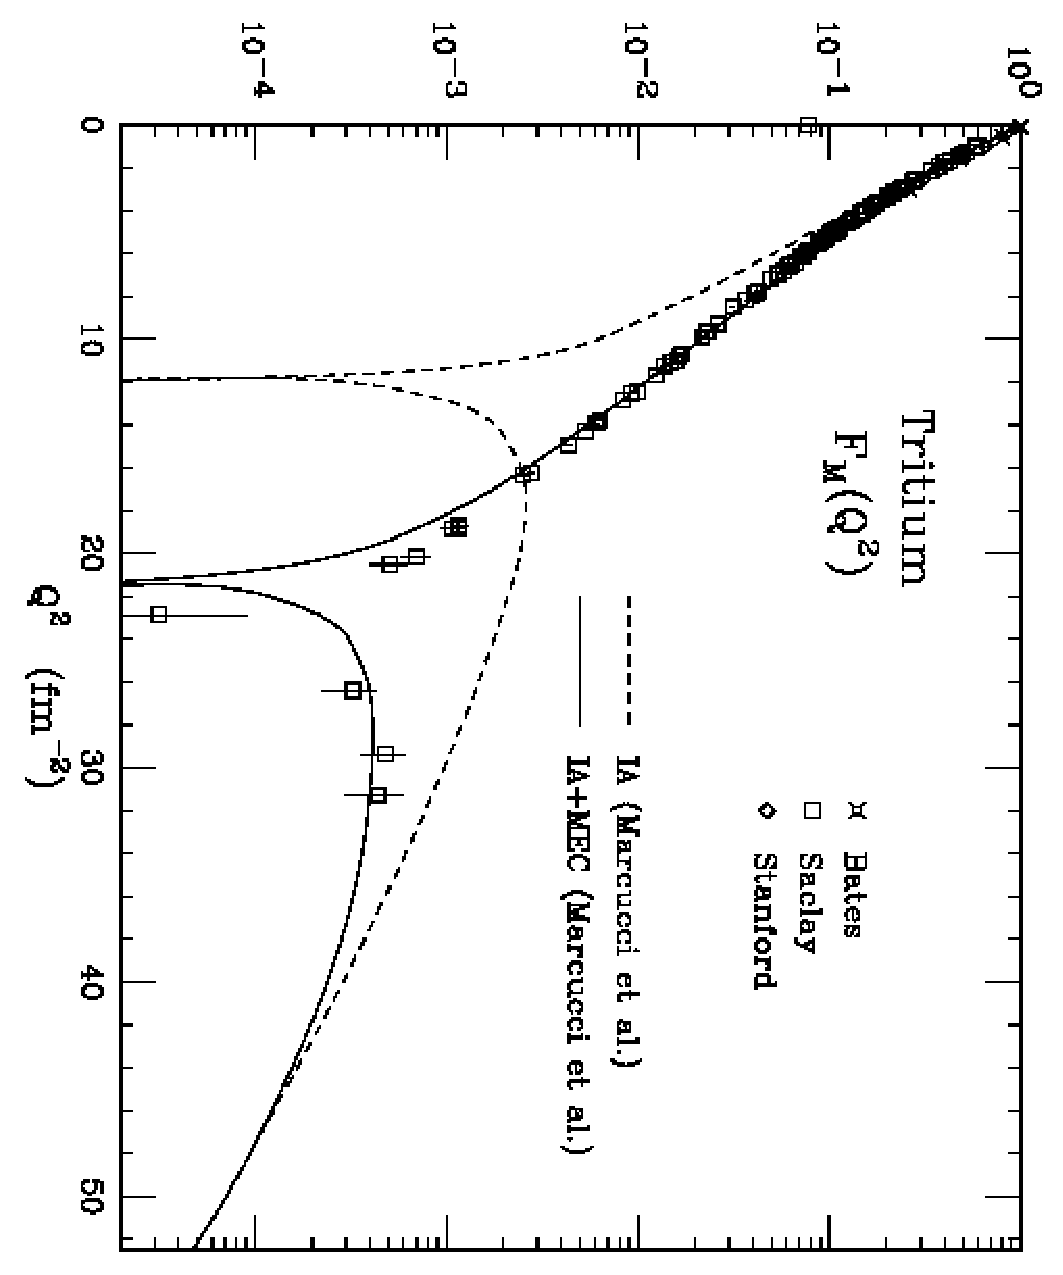
\includegraphics[angle=90, scale=0.65]{./chap2-exp/fig/tritium_past.eps}
%  \end{center}
%  \caption[Tritium Magnetic Form Factor Past Data]{
%    \footnotesize Tritium Mag. Form Factor past data.
%  }
%  \label{fig:TritiumM}
%\end{figure}
%
%Use the label name to refer to  Figure  ~\ref{fig:TritiumM}.
%
%
%\subsection{Second Subsection  Title}
%
%Subsection text..........
%
%
%
%\subsubsection{First Subsubsection}
%
%This is a subsubsection.
%
%
%
%\subsubsection{Second Subsubsection}
%
%This another  subsubsection.

\section{CEBAF Accelerator}

The Continuous Electron Beam Accelerator Facility (CEBAF) accelerator is a recirculating accelerator at Thomas Jefferson National Accelerator Facility (JLab). That is, there are two linear accelerators (linacs) connected by recirculation arcs. CEBAF has recently undergone an upgrade which increased the maximum possible energy to 12 GeV (to Hall D). The 12-GeV configuration of CEBAF can be seen in Figure \ref{fig:cebaf}. Electrons traveling through both linacs a single time is called a ``pass''. Halls A, B, and C are capable of receiving up to 5-pass beam; Hall D can receive up to 5.5-pass beam. The beam provided is Continuous Wave (CW), comprised of a steady stream of electrons, rather than many electrons in short pulses.

\begin{figure}[h]
\begin{center}
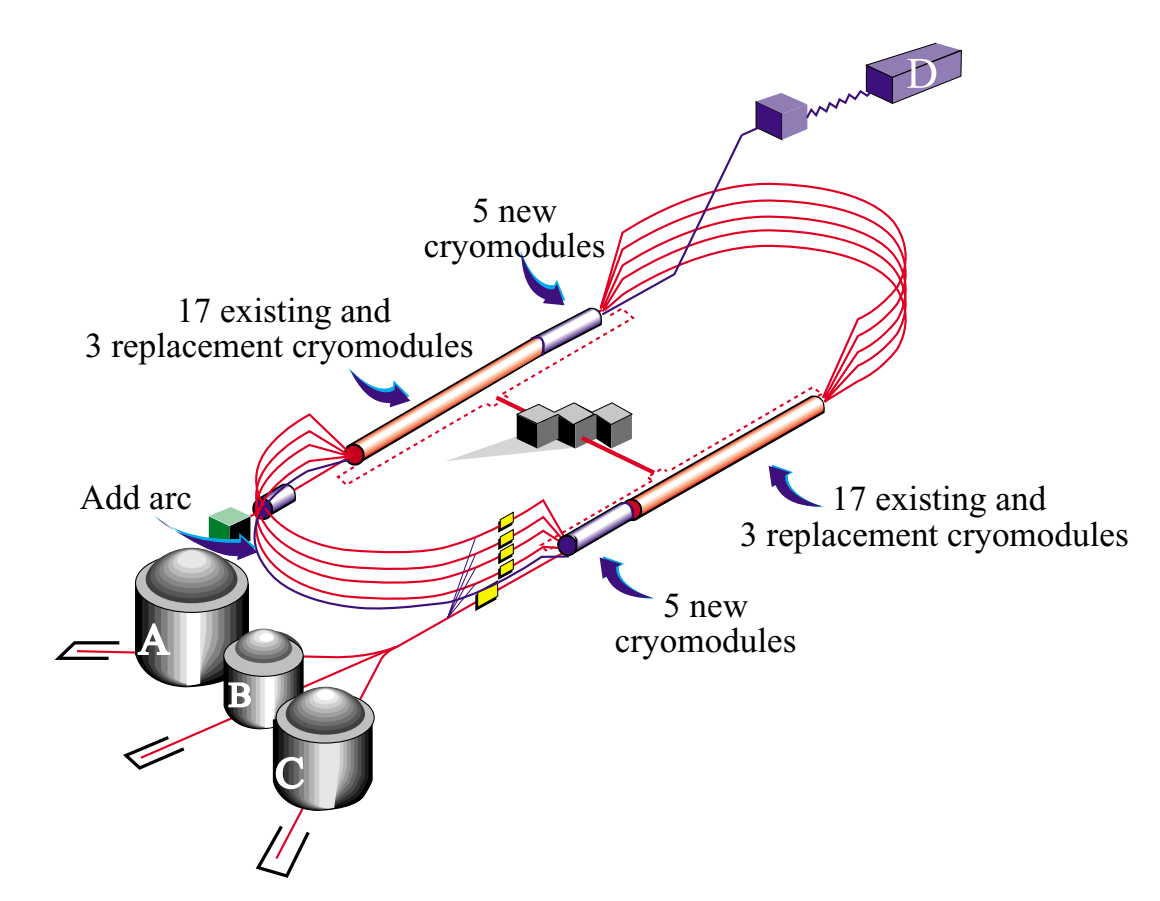
\includegraphics[width=0.7\textwidth]{./setup/fig/cebaf.png}
\caption{The current 12-GeV configuration of the CEBAF accelerator with the upgrades that were made from the 6-GeV configuration \cite{12gevWP}.}
\label{fig:cebaf}
\end{center}
\end{figure}


%Put this in order they appear in beamline?
\section{Beamline Components}

When the electrons from the CEBAF Accelerator have circulated the desired number of passes, they then enter the Hall A beamline. The Hall A Beamline has several measurement devices that allow the experimenter to fully understand the beam that is being delivered to the hall. A schematic of Hall A with the beamline components that are present in the hall can be seen in Figure \ref{fig:ha_overhead}. High beam quality and understanding the beams characteristics are critical for accurate analysis of an experiment. In the MARATHON experiment, the critical beamline components (which will be described in this section) are:

\begin{itemize}
	\item Beam Arc Energy Measurement
	\item Beam Current Monitor
	\item Raster
	\item Beam Position Monitor
\end{itemize}

\begin{figure}[h]
\begin{center}
	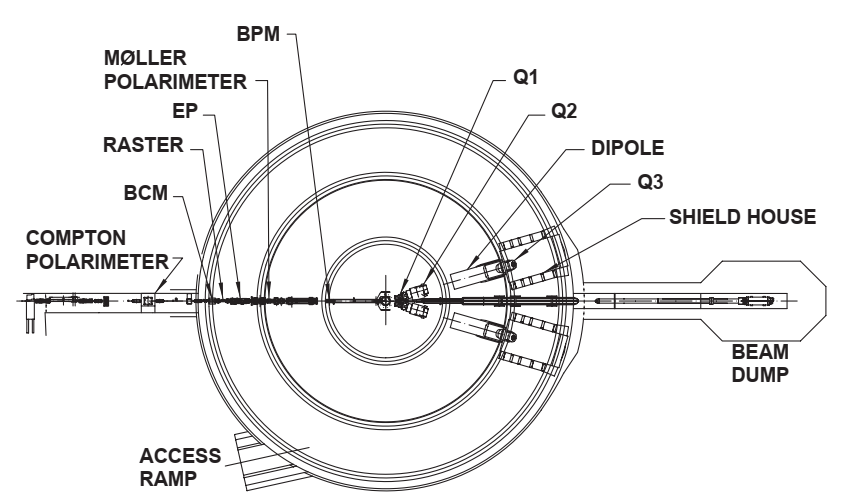
\includegraphics[width=0.7\textwidth]{./setup/fig/HallA_overhead.png}
	\caption{An overhead schematic of Hall A \cite{HANIM}.}
	\label{fig:ha_overhead}
\end{center}
\end{figure}

\subsection{Arc Energy Measurement}

Knowing the energy of the beam into the hall is critical for understanding the kinematics of the scattered electrons. This is done by measuring the deflection of the beam when passing through a series of eight dipoles in the beam arc leading to the hall. This measurement requires wire scanners to measure the bend angle of the beam through the arc and a probe to measure the magnetic field integral of the dipole magnets. 

The wire scanners are ``harps'' in the beamline, two before and two after the arc. A harp consists of three tungsten wires that are introduced sequentially into the path of the beam using a stepper motor. When the beam is incident on a wire, an electromagnetic shower is induced on the wire which is read by a PMT. By determining when each wire is struck by the beam, the position of the beam can be determined very accurately. Using two harps in each position also allows for beam direction measurement. Using a harp is a destructive measurement. 

\begin{figure}[h]
\begin{center}
	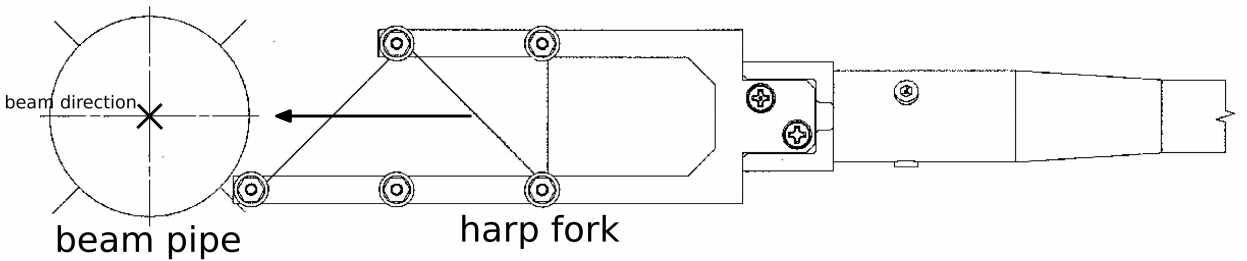
\includegraphics[width=\textwidth]{./setup/fig/harp.png}
	\caption{A schematic drawing of a harp scanner. The harp is introduced into the beamline with a stepper motor. The three wires create a signal when they interact with the beam, allowing for highly accurate beam position determination. The wires touching the beam is a destructive measurement \cite{harp_schem}.}
\end{center}
\end{figure}

The field integral is measured on a ninth reference dipole that is not in the beamline. This ninth dipole is identical to the eight dipoles in the arc and is powered in series with the other dipoles. Measuring the field integral of the dipole requires a probe to be within the magnet, necessitating the use of this reference magnet \cite{HASEM}.

After measuring the field integral $\int\vec{B}\cdot\vec{d}l$ (in Tm) and angle $\theta$ (in radians), the momentum (in GeV/$c$) can be calculated with
\begin{equation}
	p = k\frac{\int\vec{B}\cdot\vec{d}l}{\theta}
\end{equation}
where $k=0.299792$ GeV$\cdot$rad/$\left(\text{Tm}c\right)$.

\subsection{Beam Current Monitor}

The Hall A Beam Current Monitor (BCM) is comprised of an Unser monitor and two RF cavities. The Unser, a Parametric Current Transformer, provides an absolute reference for the RF cavities. Each RF cavity is tuned to the frequency of the beam (1.497 GHz). The resonance then produces a voltage proportional to the beam current. The signals are then split to be either sampled or integrated. The sampled signal outputs the RMS of the voltage over a 1 second period. This is equivalent to the average beam current for that second. The signal that is integrated is first sent to an RMS-to-DC converter which is then fed to a Voltage-to-Frequency converter. This signal is then sent to a scalar that accumulates over a run. The final scalar value is proportional to the total accumulated charge in the run.

\subsubsection{Beam Current Monitor Calibration}

The Unser is calibrated by putting a current on a wire that is inside of the Unser cavity and measuring the signal that is output. The calibration of the Unser drifts quite quickly, so it is used to calibrate the RF cavities but cannot be used for long-term monitoring. Once the Unser is properly calibrated, the reading can be used to determine the calibration for the RF cavities. The RF cavity calibration is a linear relationship between the RF cavity reading and the beam current.

\subsection{Raster}

\begin{figure}[h]
\begin{center}
	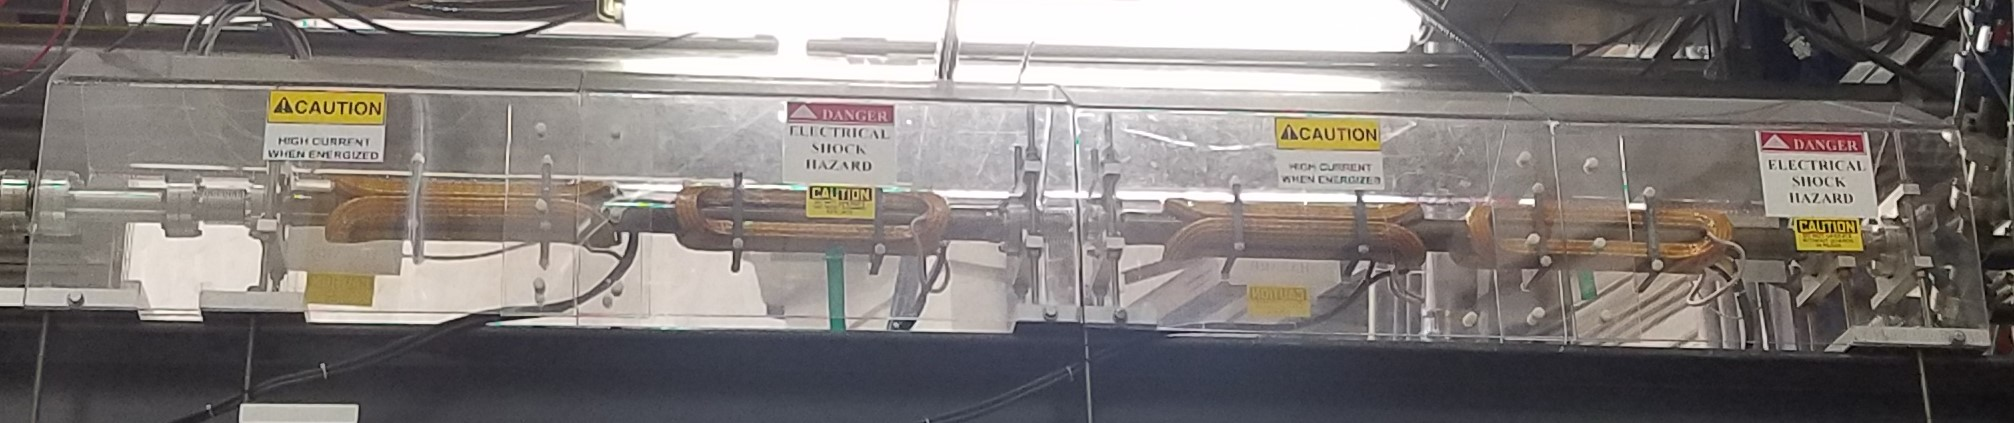
\includegraphics[width=\textwidth]{./setup/fig/raster_pic.jpg}
	\caption{The Hall A raster consists of four dipole magnets on the beamline}
	\label{fig:rasterpic}
\end{center}
\end{figure}

When the beam enters Hall A, it has very little spread, meaning that all of the electrons will strike the target in one small location (typically 80-200 $\mu$m). This poses an issue for the targets in use. Depending on the beam current in use, a localized beam spot can significantly heat up the target. In the case of solid targets, this risks melting the target. For gas targets, there is a potential for cell rupture. The raster, shown in Figure \ref{fig:rasterpic}, exists in the beamline to mitigate this risk by spreading the beam over a larger area on the target. The larger beam spread helps to reduce localized heating of the target due to the incident beam. The raster is a set of four dipole magnets: two for steering horizontally (x) and two for steering vertically (y) \cite{Bob}.

\begin{figure}[h]
\begin{center}
	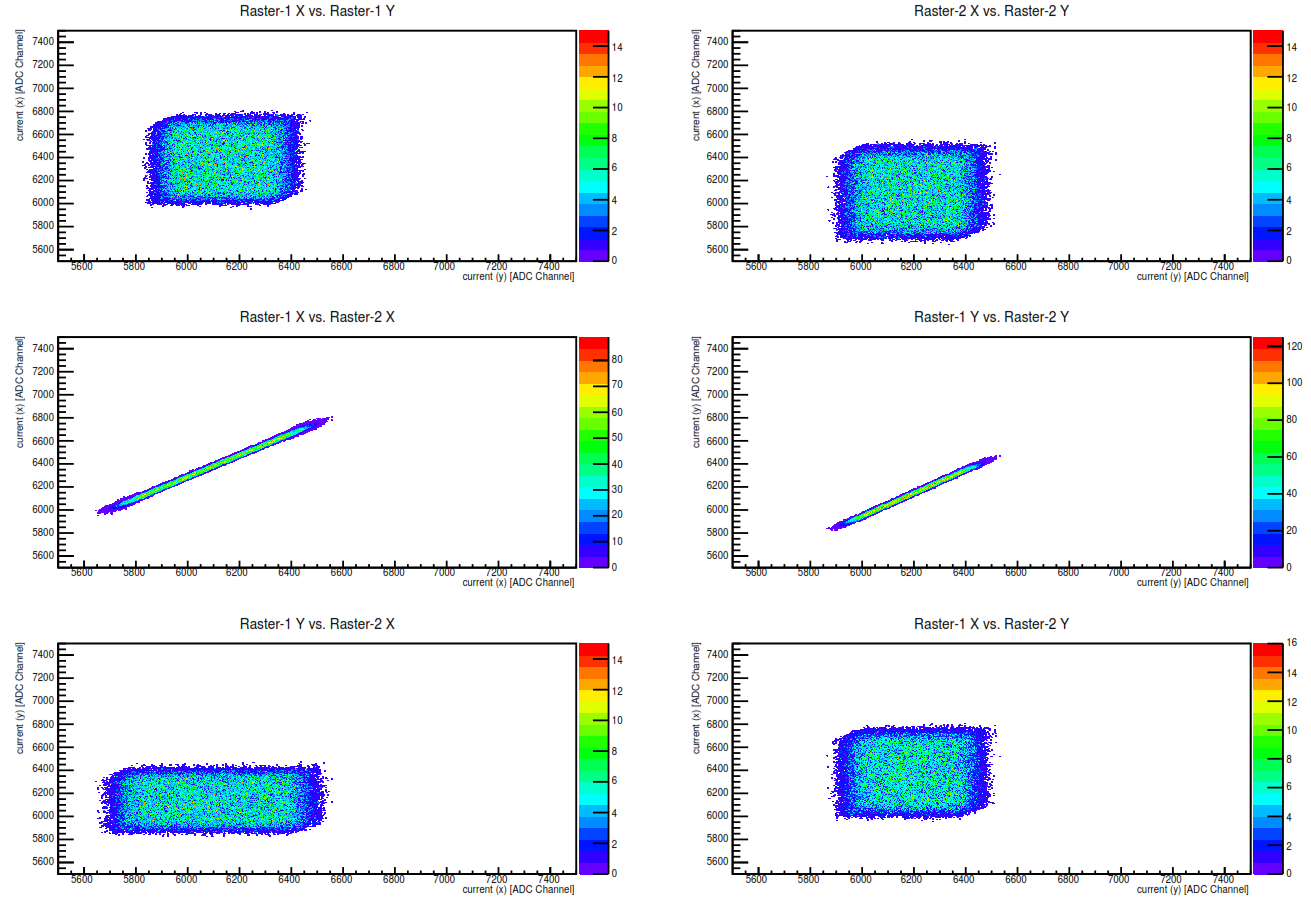
\includegraphics[width=0.7\textwidth]{./setup/fig/raster_sync.png}
	\caption{The X and Y raster pairs are each synced to produce the maximum kick. The X and Y directions are uncorrelated so that the beam travels uniformly over the target.}
	\label{fig:raster}
\end{center}
\end{figure}

\begin{figure}[h!]
\begin{center}
	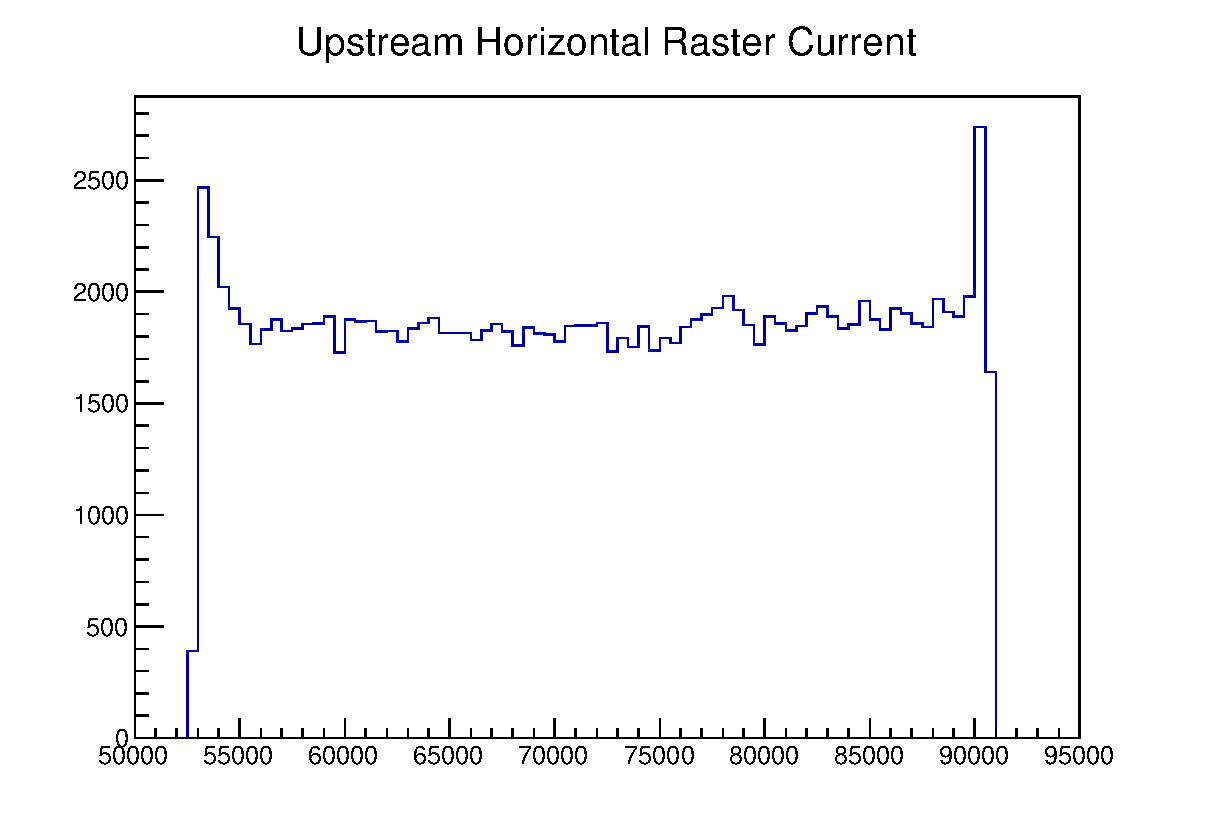
\includegraphics[width=0.7\textwidth]{./setup/fig/ex_rast.eps}
	\caption{An example of a raster current spectrum. The range and size will change with ADCs used, beam energy, and raster size. The shape should always stay the same. The ``bedposts'' on the edges are due to rounding of the triangular waveform by a low-pass filter.}
	\label{fig:exrast}
\end{center}
\end{figure}

The magnet pairs that work in the same direction are synced, which ensures that they maximize the beam spread and do not work against each other. This characteristic can be seen in Figure \ref{fig:raster}. Each raster magnet is powered by a triangle wave of different frequencies to minimize harmonics. The horizontal rasters are set to 24.5 kHz and the vertical rasters are set to 25 kHz \cite{rast_current}. The triangle wave ensures that equal time is spent at all points in the rastered area. Figure \ref{fig:exrast} shows a typical raster spectrum as recorded by the High Resolution Spectrometer (HRS).

\subsubsection{Raster Calibration}

The raster is calibrated by defining a line that maps the raster current to positions at each BPM and the target. To do this, the slope and intercept of this line had to be determined. The slope corresponds to the conversion of raster current to position displacement. The intercept is then determined from the central position that the beam is displaced from. This section will be a general presentation of the techniques used to calibrate the raster. For a more in-depth discussion of how the raster was calibrated, see Appendix \ref{raster_appendix}.

For the horizontal raster, this was done by optimizing the reconstructed z-vertex on the target. When properly calibrated, there should be no correlation between the horizontal raster and the z-vertex. Linear interpolation between two ``bad'' calibrations is a simple way to determine the correct calibration slope.

The veritcal raster could be calibrated in a similar way by minimizing the correlation between the vertical raster and a known momentum phenomena (i.e. a $W^2$ peak). Unfortunately, such a feature does not exist within the kinematics of MARATHON data. The vertical calibration was determined using the carbon hole target. The hole is known to be $2$mm diameter. By using the raster data, the hole can be fit in order to determine the vertical calibration slope.

The intercepts are determined by looking at the mean BPM position readings and projecting these to the target. This position will correspond to the mean value of the rasters as well. Using the beam position, raster current, and calibration slope the calibration intercept can easily be determined.

\subsection{Beam Position Monitors}

The Beam Position Monitors (BPMs) are a pair of measurement devices that consist of four sensing wires, as diagrammed in Figure \ref{fig:bpm}. These four sensing wires are tuned to the fundamental frequency of the beam. Using the signal received from each wire, the experimenter can reconstruct the position of the beam as it passed the BPM. Using both BPMs in conjunction allows the experimenter to determine the beam trajectory and where the electrons are incident on the target.

\begin{figure}[h]
\begin{center}
	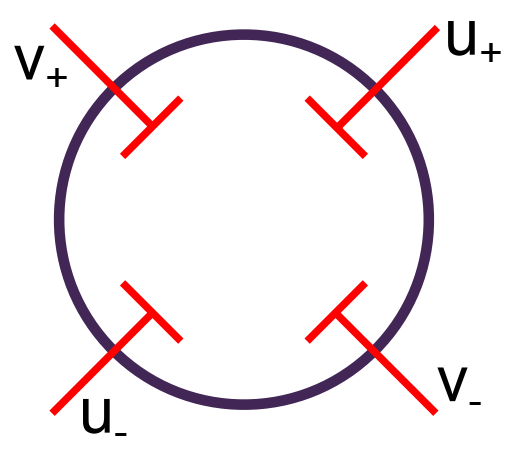
\includegraphics[width=0.5\textwidth]{./setup/fig/bpm.png}
	\caption{The BPM uses four sensing wires to determine the beam position. Since the wires do not actually touch the beam, this measurement can be done during data taking \cite{harp_schem}.}
	\label{fig:bpm}
\end{center}
\end{figure}

The BPM electronics have a phase lag between the BPM measurement and the actual beam position. This means that the BPMs cannot provide position information on an event-by-event basis. However, they do provide a measure of the average position of the beam with a record of beam spread. This information is a critical component to calibrating the raster to provide accurate event-by-event position information.

\subsubsection{Beam Position Monitor Calibration}

Using the BPMs alone provides only a reference position. The BPMs must be calibrated using a harp in order to measure the absolute beam position. This is done by a ``bullseye scan'', shown in Figure \ref{fig:bullseye}. This is accomplished by moving the beam to five positions corresponding to the corners of a square and the center of the square. The harp will give an absolute position measurement of the beam at these positions. The BPMs are also used to measure the beam position as well. The calibration is done by determining the transformation coefficients that will convert the BPM signals to the positions returned by the harps.

\begin{figure}
\begin{center}
	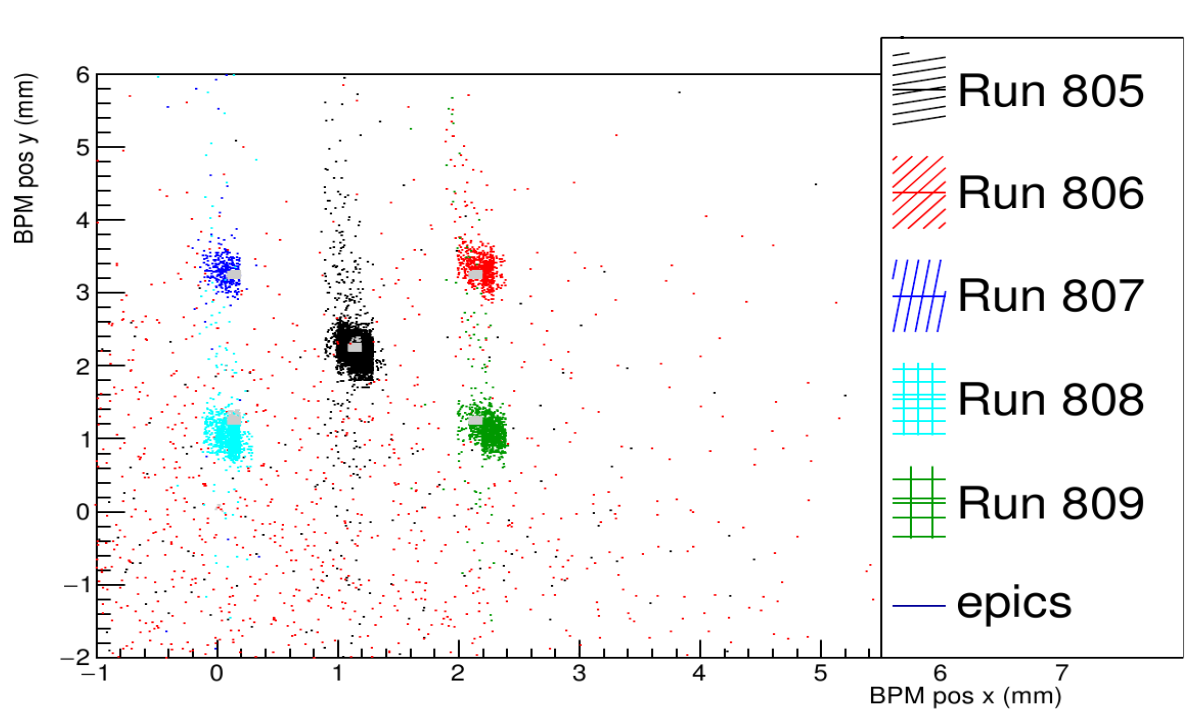
\includegraphics[width=0.7\textwidth]{./setup/fig/bullseye_scan.png}
	\caption{A bullseye scan maps five positions of the beam with the harp, shown as runs 805-809. The BPM calibration is then adjusted to make the reconstructed beam position, shown as gray blocks, match the harp data.}
	\label{fig:bullseye}
\end{center}
\end{figure}
%Put this in order they appear in beamline?
\section{Tritium Target System}

When the beam reaches the center of Hall A, it will meet the target. Here the beam will either interact with the target and scatter, allowing for detection of events that are within the acceptance of the spectrometer, or pass through the target and be deposited in the beam dump. Figure \ref{fig:ha_side} shows a side view of the hall, with the beam going from left to right. This view of the hall clearly shows these two possible paths for the beam (along the dashed line). For clarity, the spectrometer is drawn at a $0\degree$ scattering angle, which is not a position the spectrometer can physically occupy.

\begin{figure}
\begin{center}
	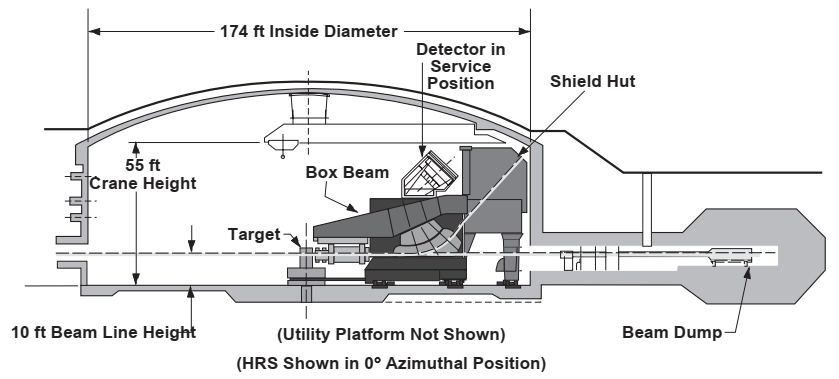
\includegraphics[width=.8\textwidth]{./setup/fig/HallA_side.png}
	\caption{A side-view schematic of Hall A showing the beamline, target, High Resolution Spectrometers, and Beam Dump. The beam will either interact with the target or pass through to the beam dump.\cite{HANIM}}
	\label{fig:ha_side}
\end{center}
\end{figure}

\subsection{Gas Cell Design}
\label{sec:gas_cell}
The gas targets used in this experiment were housed in a specially designed cell. This cell deviates from typical cells used in Hall A in that the gas is not circulated. The need for such a design is to meet safety protocols when using a tritium target, specifically to minimize tritium material and to mitigate the risk of tritium leakage.

The target cells are 25 centimeters long and made of Aluminum 7075. The cells are sealed and utilize conductive cooling. The beam heating of the aluminum is approximately 11W. This heat is recovered by a copper heat sink that is actively cooled by 15K helium gas.\cite{cell_design} Figure \ref{fig:3d_cell} shows a 3-dimensional rendering of the target cell. The beam comes in from the bottom-left and passes through the center of the target along the length.

\begin{figure}[h]
\begin{center}
	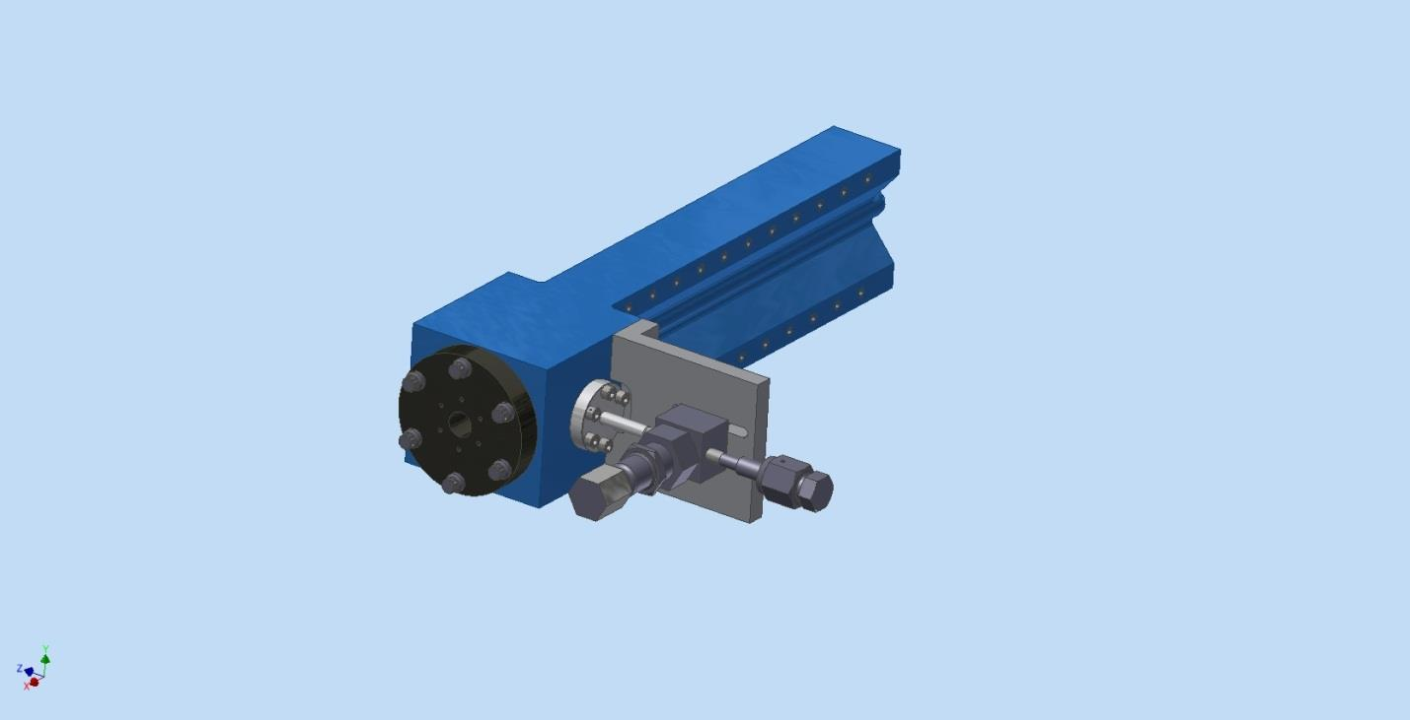
\includegraphics[width=0.7\textwidth]{./setup/fig/targ_cell.png}
	\caption{3D rendering of the target cell. The black circular plate in the front is the upstream window of the cell.\cite{cell_design}}
	\label{fig:3d_cell}
\end{center}
\end{figure}

The lack of gas circulation allows for localized heating of the gas in the cell. This is caused by the energy being deposited into the gas by the incident beam. The heating causes a density change in the gas changing the effective target thickness. This characteristic must be addressed in the analysis of gas target data and is discussed in further detail in Section \ref{sec:boiling}.

\subsection{Target Ladder}
The MARATHON target ladder can be seen in Figure \ref{fig:target}. This target ladder contained five targets that utilized the gas cell design described in the previous subsection. These are:
\begin{itemize}
	\item Tritium
	\item Deuterium
	\item Hydrogen
	\item Helium-3
	\item Empty Cell
\end{itemize}

The cells that contain gas (i.e. all of the above except the empty target) are used for studying the physics goals of the MARATHON experiment. In particular, Helium-3 and Deuterium are the focus of this thesis. Table \ref{tbl:gas_targs} lists the gas thicknesses and endcap thicknesses of the above gas targets.

\begin{table}[h]
\begin{tabular}{|l|c|c|c|}
\hline
Target & Gas Thickness $\nicefrac{\textrm{g}}{\textrm{cm}^2}$ & Entrance Window Thickness (mm) & Exit Window Thickness (mm) \\
\hline
\hline
Tritium & $77\pm0.01$ & $0.253\pm0.004$ & $0.3430.047$\\ \hline
Deuterium & $142.2\pm0.8$ & $0.215\pm0.004$ & $0.294\pm0.056$\\ \hline
Hydrogen & $70.8\pm0.4$ & $0.311\pm0.001$ & $0.330\pm0.063$\\ \hline
Helium-3 & $53.4\pm0.6$ & $0.203\pm0.007$ & $0.328\pm0.041$\\ \hline
Empty cell & $N/A$ & $0.254\pm0.0051$ & $0.279\pm0.0051$\\ \hline
\end{tabular}
\caption{Gas target thicknesses and cell wall thicknesses.\cite{targ_meas}}
\label{tbl:gas_targs}
\end{table}

In addition to the gas cells, the target ladder also contained several solid targets that are used for other studies. Those relevant to this thesis are:
\begin{itemize}
	\item 25cm Dummy
%	\item Optics Target - 11 Carbon Foils
	\item Carbon Hole - A carbon foil with a 2mm diameter hole in the center
	\item Raster Target - A ``straw'' for ensuring the beam is not coming in at an angle
%	\item Thick Aluminum - For calibrating the ion chambers
%	\item Single Carbon Foil
%	\item Titanium
%	\item Beryllium Oxide
\end{itemize}

\begin{figure}[h]
\begin{center}
	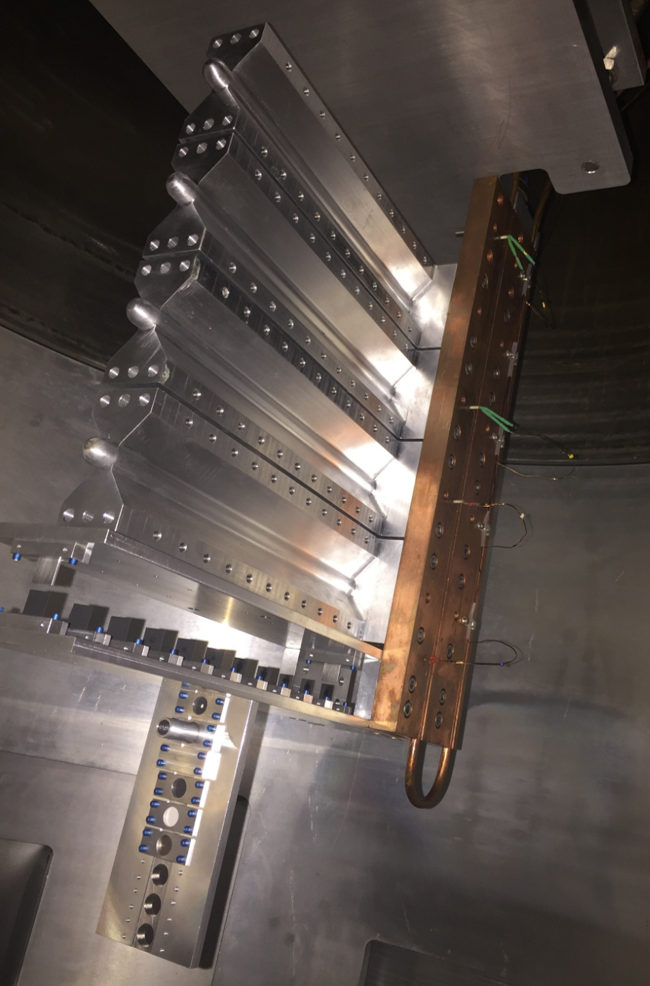
\includegraphics[width=0.4\textwidth]{./setup/fig/target.png}
	\label{fig:target}
	\caption{The MARATHON target ladder.}
\end{center}
\end{figure}

%Put in target data table: endcap thicknesses, density, fill pressure, target thickness

The Empty target is a gas cell that has a vacuum inside. The 25cm Dummy is comprised of two Aluminum 7075 foils, this is the same material as the gas cells. The foils are spaced 25cm apart, the same length as the gas cells.  Each foil is $0.3495\pm0.0006$ $g/cm^2$ thick, significantly thicker than the cell walls. These two targets are used to better understand the contribution of the gas cells to the electrons counted by the experiment. This study is discussed further in Section \ref{sec:ecc}.

The Carbon Hole target is a foil made of carbon that is $0.883\pm0.0002$ $g/cm^2$ thick with a $2mm$ diameter hole in the center. This target is used for centering the beam as well as for determining the settings needed for a $2mm$ by $2mm$ raster setting. This is also used to assist calibrating the raster as documented in Appendix \ref{app:raster_cal}.

After the beam is centered and the raster settings are determined, the Raster Target is used. This target is a ``straw'' that the beam should pass straight through. The goal of using this is to ensure that the beam is not approaching the target at an angle. If any counts are seen above background, then the beam is hitting the straw and can be assumed to be coming in at an angle that needs to be rectified. If the beam is angled, electrons would leave the physics targets before passing through all of the target material. This would significantly reduce counting rates and make it very difficult to determine the effective target thickness seen by the beam.
\section{The Hall A High Resolution Spectrometer}

Hall A has two 4 GeV/c High Resolution Spectrometers (HRSs), designated Left (LHRS) and Right (RHRS) corresponding to their orientation when looking downstream along the beam. In order to achieve Hall A's stated goal of $1\%$ absolute cross section accuracy, the HRSs were designed to have $10^{-4}$ particle momentum resolution and $0.1$ mrad in scattering angle resolution. 

Each HRS has four superconducting magnets: three cos$\left(2\theta\right)$ and a racetrack coil dipole. Utilizing a QQDQ magnet setup (named Q1, Q2, D, and Q3), each HRS has a $45\degree$ bending angle in a vertical bending plane. Each HRS has a similar, but unique, detector package that accommodates precise tracking and particle identification (PID). Figure \ref{fig:hrs_mags} shows the magnet layout of the HRSs. The setup is identical on both the Left and Right HRS.

\begin{figure}
\begin{center}
	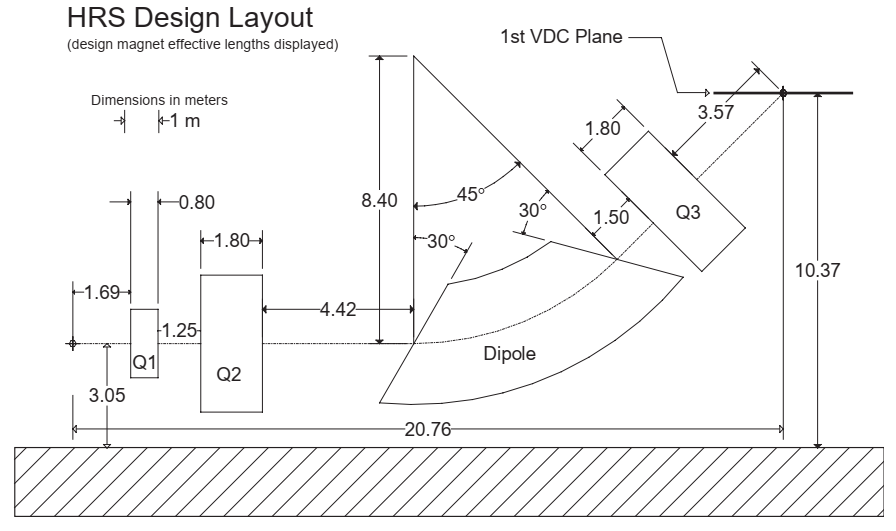
\includegraphics[width=0.8\textwidth]{./setup/fig/HRS_mags.png}
	\caption{A schematic view of the HRS magnet setup. Particles enter from the left in Q1 and then pass through the magnets exiting Q3 into the first VDC plane.\cite{HANIM}}
	\label{fig:hrs_mags}
\end{center}
\end{figure}

The two HRSs can be ran together for exclusive measurements or ran separately for inclusive measurements. MARATHON used each HRS separately in order to maximize counting rate. In particular, the RHRS was parked at the highest angle measurement as the counting rate was very slow.

Each arm consists of a pair of Vertical Drift Chambers (VDCs), two scintillator planes, a gas cherenkov, and two leaded glass calorimeters. This combination of detectors allows for fine tracking and powerful electron identification.

\subsection{Vertical Drift Chambers}

Each arm has two VDCs at the entrance to the detector stack. These detectors are used for fine tracking of particles. Drift chambers are comprised of high voltage planes, sense wires, and a gas mixture. When a particle passes through a drift chamber it ionizes the gas. The high voltage planes keep a constant electric field within the drift chamber. The sense wires are held at ground potential. The ionized gas from incident particles then drifts toward the sense wire creating a build up of charge that can be measured. Using the drift speed of ions in the field and the time that it takes for the ion to reach the sense wire, the position of the track through the VDC can be accurately determined.

The chambers used in the HRSs, as seen in Figure \ref{fig:vdcs}, are oriented parallel to the horizontal plane of the hall and $45\degree$ to the detector stack. The active area of each VDC is 2118 mm by 288 mm. The gas used is an argon (62\%) and ethane(38\%) mixture. The electric field is created by gold-plated Mylar planes spaced 13 mm apart. These planes are held at -4 kV. Each chamber has two wire planes in a UV formation, that is $90\degree$ to each other, that are separated by 335 mm. In each plane there are 368 wires with a wire spacing of 4.24 mm. This setup gives a position resolution of 100 $\mu$m and an angular resolution of 0.5 mrad.

\begin{figure}
\begin{center}
	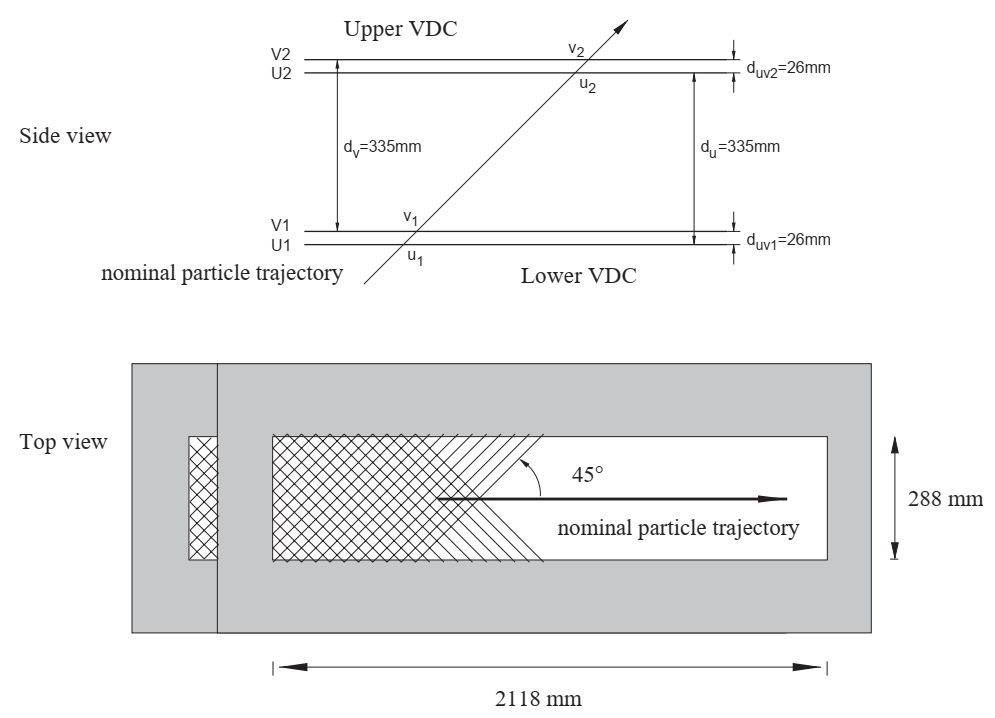
\includegraphics[width=0.8\textwidth]{./setup/fig/vdc.png}
	\caption{A schematic view of the VDCs. These are the first detectors in an HRS.\cite{HANIM}}
	\label{fig:vdcs}
\end{center}
\end{figure}

\subsection{Scintillator Planes}

Each HRS has two scintillator planes that were used for MARATHON: S0 and S2. These two planes sandwich the Gas Cherenkov. The scintillators are plastic paddles with a Photomultiplier Tube (PMT) on each end. When scintillating material is struck by a particle, it absorbs a small amount of energy and emits it as light. The light then travels through the material to the PMTs on each end. When the light reaches the PMT, it knocks electrons out of the photocathode. These electrons are accelerated through a series of exceedingly higher voltage dynodes where more electrons are released. Finally, this cascade reaches the anode with a enough electrons to create a signal that can be read in. This entire process is very quick, allowing the scintillators to be used for setting the timing of events. The time difference between the signal in the PMTs on each end allows for rough tracking.

S0 consists of a single paddle with the PMTs on located on the top and bottom. The S0 paddle made from BICRON 408 scintillating plastic which is 10 mm thick, 170 cm long, and 25 cm wide. The PMTs used are $3''$ XP2312B. There is a trade-off in timing resolution when using a large paddle. The timing resolution of S0 is approximately $0.2ns$.

S2 consists of 16 paddles with the PMTs on the left and right. Each paddle is made from fast plastic scintillator EJ-230 and is 2 inches thick, 17 inches long, and 5.5 inches wide. The paddles are pressed together with a 60 pound force in order to minimize any space between the paddles. The PMTs used are $2''$ Photonis 2282B. Figure \ref{fig:s2} shows the layout of the S2 scintillator plane. In this drawing, particles would pass through the plane of the page. The timing resolution of S2 has been measured to be smaller than $150ps$.

\begin{figure}
\begin{center}
	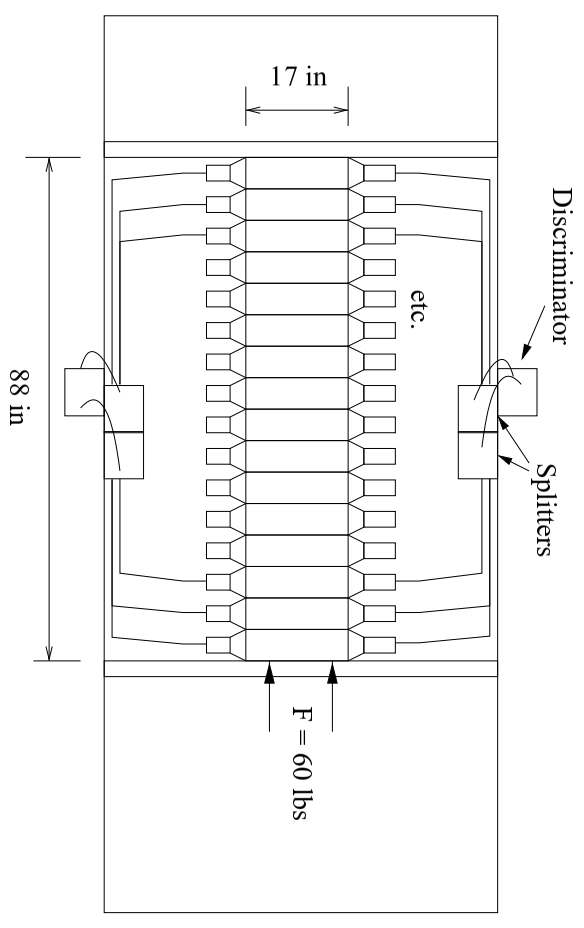
\includegraphics[width=0.3\textwidth]{./setup/fig/s2.png}
	\caption{A schematic drawing of the S2 scintillator plane.\cite{HASEM}}
	\label{fig:s2}
\end{center}
\end{figure}

The signals measured in the scintillators form the basis for the HRS trigger. Since S2 has high time resolution, it serves to set the timing of the event. Proper event timing is critical for the VDCs to accurately track a particle.

\subsection{Gas Cherenkov}

The Gas Cherenkov is the first PID detector in the HRS. A gas cherenkov detector functions by observing cherenkov radiation from incident particles. Cherenkov radiation is light emitted by a particle that is traveling faster than the phase velocity of light in a medium. The cherenkov radiation is emitted as an ``electromagnetic shock wave'' in the wake of the particle that is then guided to PMTs by mirrors. This property allows a gas cherenkov detector to exclude low momentum particles.\cite{Leo}

The Cherenkov chamber is filled with C02 at atmospheric pressure. This gas gives a 4.8 GeV/\textit{c}  momentum threshold for pion detection. This provides very efficient rejection of pions, as the HRSs have a momentum acceptance set much lower than that. Each chamber has ten spherical mirrors with focal length 80 cm each aimed at a PMT (Burle 8854). The radiator length is 80 cm for the LHRS and 130 cm for the RHRS.

All of these things means that analyzing the sum of all PMT signals allows for very efficient discernment between electrons and pions.

\subsection{Leaded Glass Calorimeters}

Both arms have two leaded glass calorimeters, known as the preshower and shower detectors. When a particle enters a calorimeter, it interacts with the material by depositing energy. This energy is converted into an electromagnetic shower of photons which are detected by PMTs attached to the glass blocks. How much energy is deposited is dependent on the particle and its radiation length within the material. In the case of the HRSs, the calorimeters are thick enough that electrons will completely deposit all of their energy into the preshower and shower detectors. Each HRS has a slightly different configuration for the calorimeters.

In the LHRS, the preshower and shower blocks are all perpendicular to the path of the particle. Both layers have are comprised of 34 blocks at alternate in size between 15 cm x 15 cm x 30 cm and 15 cm x 15 cm x 35 cm.

In the RHRS, the preshower blocks are perpendicular to the path of the particle while the shower blocks are parallel to the path of the particle. The preshower layer is composed of 48 blocks that measure 10 cm x 10 cm x 35 cm. The shower layer is composed of 80 blocks that measure 15 cm x 15 cm x 35 cm.

The signal from the calorimeters is directly correlated to the energy of the particle that was detected. Typically for PID, a measure of $E/p$ is used, that is the ratio of energy to momentum of the detected particle. This allows for very efficient identification of particles because electrons will peak around 1 and larger particles will have a much lower ratio.

\begin{figure}
\begin{center}
	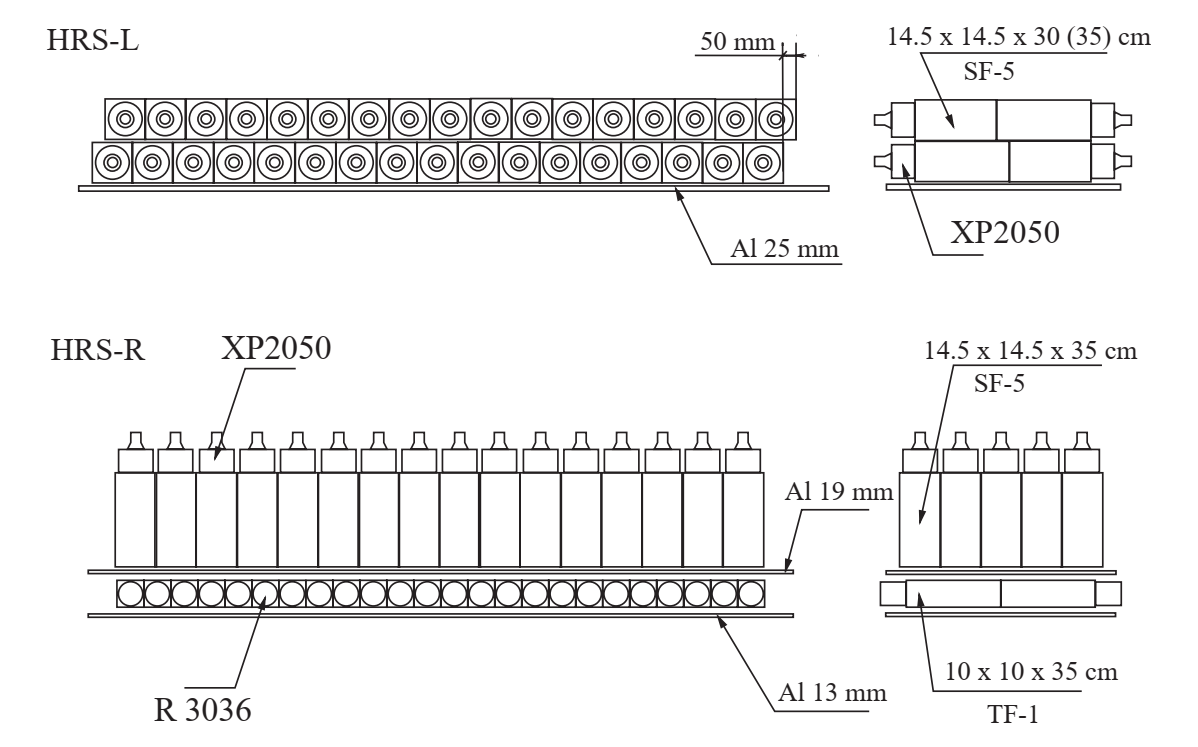
\includegraphics[width=0.8\textwidth]{./setup/fig/shower_layout.png}
	\caption{Layout of the shower blocks. Particles enter from the bottom of the page. Left is top-view. Right is side-view. \cite{HANIM}}
	\label{shower_layout}
\end{center}
\end{figure}

\subsection{Trigger}

The HRSs read in data from the described detectors through a combination of Fastbus ADCs and TDCs and VME Flash ADCs. A Trigger Supervisor (TS) unit is used to distribute a trigger signal to this hardware. This trigger signals the ADCs and TDCs to record this signal and send it to be written. This process is overseen by CEBAF Online Data Acquisition (CODA) software written at JLab. The CODA software communicates with the TS crate to signal when it is ready to receive data and that triggers should begin being processed.

In order to distribute a signal to the ADCs and TDCs, the TS unit must receive an outside trigger. A trigger is a logic signal that is generated to indicate that the data that would be recorded is potentially a ``good event''. This trigger is generated from the signals that are produced by the detectors in the HRSs.

To produce this trigger, signals received from the scintillators and cherenkov are processed by NIM electronics. First, the signals are scintillator PMT signals are ``discriminated''. Each of these signals are then passed through a discriminator which, provided the signals are large enough to exceed a set threshold signifying a real signal, converts the signal into a logic pulse. The length of these logic pulses is set to allow for timing the coincidence of these three detectors. The PMTs in each scintillator plane are then checked for coincidence, that is any signal received within a designated window of time is defined as being from the same event. In the setup for S0, both PMTs must have a signal for this process to consider there to have been an event. The S2 setup requires that any single paddle must have a signal from both PMTs in order to trigger. For the cherenkov, the PMT signals are summed and then discriminated. The logic pulses for each detector are then delayed to allow for timing of coincidence between detectors. The need for delaying the signals is due to the varying length of cables from the detectors to the processing hardware.

These logic signals are finally combined into four different triggers:
\begin{itemize}
	\item S0 \textbar\textbar{} S2
	\item S0 \&\& S2
	\item (S0 \textbar\textbar{} S2) \&\& Cherenkov
	\item (S0 \&\& S2) \&\& Cherenkov
\end{itemize}
Ultimately, the final three of these triggers were used in the experiment. A schematic of formation of these signals can be seen in Figure \ref{fig:trig_schem}. In the formation of these triggers, the scintillators are used to set the timing for the TDCs. Particularly, S2 always sets the timing of the trigger since it has the highest timing resolution. In the case of the triggers where S0 and S2 are ``OR'd'', S0 will set the timing in the absence of an S2 signal.

\begin{figure}
\begin{center}
	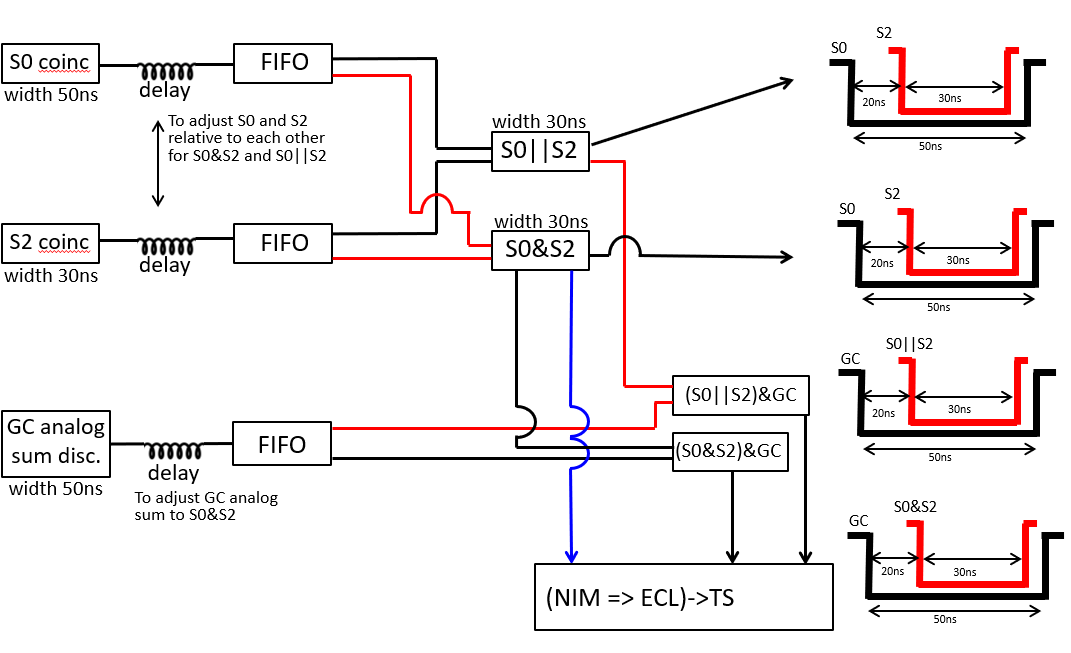
\includegraphics[width=\textwidth]{./setup/fig/trigger_diagram.png}
	\caption{A schematic diagram of the trigger setup for MARATHON. In this diagram ``disc.'' stands for discriminator. ``FIFO'' stands for ``Fan in fan out'', which is a unit that takes a signal and then outputs it to multiple channels. ``NIM=$>$ECL'' denotes the conversion from NIM to ECL logic standards which is necessary to interface with the Trigger Supervisor.\cite{Rey}}
	\label{fig:trig_schem}
\end{center}
\end{figure}
